% !Mode:: "TeX:UTF-8"
\documentclass[runningheads,a4paper]{llncs}

%\usepackage{aaai17}
\usepackage{times}
\usepackage{helvet}
\usepackage{courier}
\frenchspacing
\setlength{\pdfpagewidth}{8.5in}
\setlength{\pdfpageheight}{11in}

\let\proof\relax
\let\endproof\relax
\usepackage{amsthm}%used for theorem and definition
%\usepackage{showframe}%show the margin
%\usepackage{ulem}%used for uwave
\usepackage{comment}
\usepackage{subfigure}
\usepackage{enumitem}
\usepackage[ruled,vlined,linesnumbered]{algorithm2e}
\usepackage{algorithmic}

%================================================
%% make a tight section title
%% Save the class definition of \subparagraph
\let\llncssubparagraph\subparagraph
%% Provide a definition to \subparagraph to keep titlesec happy
\let\subparagraph\paragraph
%% Load titlesec
\usepackage[compact]{titlesec}
%% Revert \subparagraph to the llncs definition
\let\subparagraph\llncssubparagraph
\usepackage[compact]{titlesec}% shrink all the whitespace around section headings
%================================================


\usepackage{bm}%used for bm
\usepackage{graphics} % used for scalebox
\usepackage{graphicx}
\usepackage{amsmath} %used for maths symbols and the checkmark
\usepackage{amssymb}%used for empty set symbol
\usepackage{threeparttable} % used for footnotes in table
\usepackage{booktabs} %used for tnote
\usepackage{url} %used for url

\usepackage{makecell}

%Chinese
\usepackage{CJKutf8}
\inputencoding{utf8}

%================================================
%Definition
\newtheorem{thm}{Theorem}

\newtheoremstyle{exampstyle}
  {0pt} % Space above
  {0pt} % Space below
  {} % Body font
  {} % Indent amount
  {\bfseries} % Theorem head font
  {.} % Punctuation after theorem head
  {.5em} % Space after theorem head
  {} % Theorem head spec (can be left empty, meaning `normal')

\theoremstyle{exampstyle}
\newtheorem{rmkWithoutSpacing}[thm]{Definition}
%================================================


%================================================
%highlight
\usepackage{color,soul}%used for hl
\newcommand{\hlgreen}[1]{
	\sethlcolor{green}
	\hl{#1}
	\sethlcolor{yellow}
}%used for highlight, but set the color as green
%================================================
%================================================

%================================
%中文
\inputencoding{utf8}
\newcommand{\chinese}[1]{
	\begin{CJK*}{UTF8}{gbsn}
	#1	
	\end{CJK*}
}
%================================

\usepackage{multirow}% for table

\newtheorem{rmk}{Definition}% definition

%used for quotes
\usepackage{epigraph}
\setlength\epigraphwidth{\columnwidth}
\setlength\epigraphrule{0pt}

\usepackage{array}
\newcolumntype{L}[1]{>{\raggedright\let\newline\\\arraybackslash\hspace{0pt}}m{#1}}
\newcolumntype{C}[1]{>{\centering\let\newline\\\arraybackslash\hspace{0pt}}m{#1}}
\newcolumntype{R}[1]{>{\raggedleft\let\newline\\\arraybackslash\hspace{0pt}}m{#1}}

\usepackage{hyperref}
\setcounter{secnumdepth}{2}  
 \begin{document}
% The file aaai.sty is the style file for AAAI Press 
% proceedings, working notes, and technical reports.
%
\title{Category-Level Transfer Learning from Knowledge Base to Microblog Stream for Accurate Event Detection}
\titlerunning{Transfer Learning for Accurate Event Detection\ }
\author{Weijing Huang\inst{1} \and Wei Chen\inst{1} \thanks{Corresponding author.} \and Tengjiao Wang\inst{1} \and Yazhou Wang\inst{1} }
\institute{Key Laboratory of High Confidence Software Technologies (Ministry of Education), EECS, Peking University, Beijing, China \\ 
\path{huangwaleking@gmail.com,{pekingchenwei,tjwang}@pku.edu.cn}\\ 
\path{pkuwangyz@gmail.com}
}

\maketitle
% BEGIN
% To Proceeding Editors:
% Special codes there for remove page numbers in the LaTeX documents
\thispagestyle{empty}
\pagestyle{empty}
%
% END


\begin{abstract}
Many web applications need the accurate event detection technique on microblog stream. 
But the accuracy of existing methods are still challenged by microblog's short length and high noise. 
We develop a novel category-level transfer learning method \textsc{TransDetector} to deal with the task.  
\textsc{TransDetector} bases on two facts, that microblog is short but can be enriched by knowledge base semantically with transfer learning; and events can be detected more accurately on microblogs with richer semantics.
%文本短,建模很困难;直接做迁移学习困难,两者的组织结构不同,如何从精心构造的知识库迁移到微博是一个很大的挑战。
%所以我们提出了Category-Level Transfer Learning ...
The following contributions are made in \textsc{TransDetector}.
(1) We propose a structure-guided category-level topics extraction method, which exploits the knowledge base's hierarchical structure to extract categories' highly correlated topics. 
(2) We develop a probabilistic model CTrans-LDA for category-level transfer learning, which utilizes the word co-occurrences and transfers the knowledge base's category-level topics into microblogs. 
%Hence, word time series are expanded as category-pivot word time series.
(3) Events are detected accurately on category-level word time series, due to richer semantics and less noise. 
(4) Experiment verifies the quality of category-level topics extracted from knowledge base, and the further study on the benchmark \textit{Edinburgh twitter corpus} validates the effectiveness of our proposed transfer learning method for event detection.
\textsc{TransDetector} achieves high accuracy, promoting the precision by 9\% without  sacrificing the recall rate.
%另外,我们还标注了事件,使其语义可理解。以及LTDetector是efficient的。

\end{abstract}

\section{Introduction}
Many web applications need the accurate event detection technique on microblog stream, such as public opinion analysis\cite{thelwall2011sentiment}, public security\cite{Li:2012gw}, and disaster response\cite{Yin:2012ht}, etc.
Although event detection has been a research topic for a long while\cite{allan1998topic}, event detection in microblog stream is still challenging\cite{atefeh2015survey}.
According to \cite{huang2016probabilistic}, the characteristics of microblog, which is fast changing, high noise, and short length, raise the challenge.

Knowledge base can be a good supplementary for event detection on microblog stream to address these challenges.
Different from the not-well-organized microblog stream, knowledge base (e.g. Wikipedia) is constructed elaborately and contains rich information. 
For example, the microblog message ``Possible Ft. Hood Attack Thwarted (2011-07-28)'' is short, but still comprehensible because the words ``\textit{Ft. Hood}" is included in the wiki page ``\textit{Ft. Hood}", and belongs to the category ``\textit{Military}'' at a higher conceptual level.
By regarding these wiki information and the word \textit{attack} (also highly related to \textit{Military}), the model easily understands the example tweet is about something related to \textit{Military}.
In other words, knowledge base enriches the linkages between words and concepts, and provides more comprehensive context for microblogs.
Since the transfer learning\cite{pan2010survey} aims at utilizing the extra information stored in the source dataset to benefit the target dataset, it provides a feasible way to enhance the event detection in microblog stream.
Taking the below Figure \ref{fig:hood} as an example, the fluctuation of time series of raw word \textit{hood} is not so obvious to reflect the event happened to the military base \textit{Ft. Hood}.
After transferring the knowledge about \textit{``Military"} into the microblog stream, the time series of word \textit{``hood"} related to \textit{``Military"} is extracted, which is more vivid to detect the event happened on July 28th, 2011.

\intextsep=1pt plus 1pt minus 1pt
\begin{figure}[h]
		\setlength{\abovecaptionskip}{0.cm}
        \setlength{\belowcaptionskip}{0.cm}
        \centering
        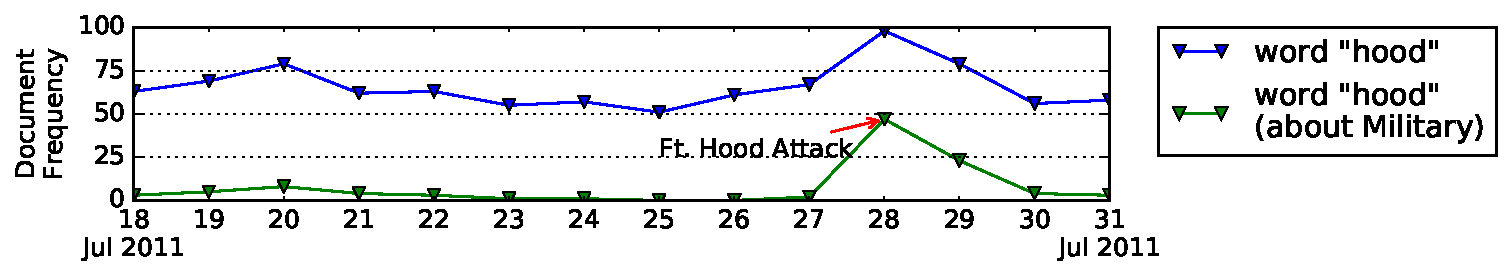
\includegraphics[width=1.0\columnwidth]{img/hood.pdf}
        \caption{The comparison of the time series between the raw word \textit{hood} and the \textit{Military} related word \textit{hood}, computed on the \textit{Edinburgh twitter corpus}\cite{petrovic2012using}. The rise of document frequency on July 28th, 2011 is corresponding to the event mentioned in \url{https://en.wikipedia.org/wiki/Fort_Hood\#2011_attack_plot}.}
        \label{fig:hood}
\end{figure}

The benefit of enriching the semantics for micorblogs is attractive, but it's non-trivial to transfer the knowledge stored in the knowledge base into microblog stream directly.
The existing RDF model\cite{klyne2006rdf} lacks an efficient quick mechanism to transfer the knowledge, since it's mainly designed for managing knowledge as tuples on graph. And the query on large graph is also very expensive\cite{huang2011scalable}, which is not suitable for the scene of quickly and accurately detecting events.
In existing methods, what meets the demand most is Twevent\cite{Twevent2012}, but it's limited in only treating Wikipedia as a looking-up table and may drop some events incorrectly.

In our paper, to balance the performance and the cost of leveraging knowledge base for event detection, we develop a novel category-level transfer learning method, namely \textsc{TransDetector}.
It consists of three phases: extracting category-level topics in knowledge base, conducting transfer learning to get category-level topics in microblog stream, and detecting events from category-level word time series, as illustrated in Figure \ref{fig:modelDesc}.
We explain the main idea of the three parts in \textsc{TransDetector}, and leave more technique details in Section \ref{sec:TransDetector}.
(1) In the \textbf{extracting} phase, we propose a structural-guided category-level topics extraction method on the knowledge base. 
It bases on the following facts. 
The knowledge base has the three fold hierarchical structure, consisting of the taxonomy graph (\textit{class} \(\rightarrow\) \textit{subclass}), the category-page bipartite graph (\textit{class} \(\rightarrow\) \textit{instance}), and the page-content map (\textit{instance} \(\rightarrow\) \textit{content}), as illustrated in Figure \ref{fig:NSinitializaton}.
In terms of concept level, the latter part is finer than the former. 
And the last page-content map goes into the detail at the word level. 
By considering these three parts together, we can extract a class or category's highly related words, and restore them in \textit{category-level topics in knowledge base}.
(2) In the \textbf{conducting transfer learning} phase, we propose a novel probabilistic model CTrans-LDA for transferring the knowledge.
CTrans-LDA works in the bayesian transfer learning way like \cite{dai2007transferring}, by utilizing the extracted \textit{category-level topics in knowledge base} as the informative priors to bridge two data domains. 
CTrans-LDA labels whether a word in a microblog message should link to a category in knowledge base, or just label it as no-category-related word.
Applying CTrans-LDA on more microblogs, it gets the \textit{category-level topics in microblog stream} and \textit{category-level word time series}.
(3) In the \textbf{detecting} phase, since the words in microblogs have been enriched semantically and the meaningless words are labeled as no-category-related, the event detection on \textit{category-level word time series} is much more accurate than other methods which don't conduct the transfer learning.
Without loss of generality, we use Wikipedia as a representative of the knowledge base in the remaining of this paper.
And the experiment on the \textit{Edinburgh twitter corpus} demonstrates the effectiveness of our proposed \textsc{TransDetector}.


\intextsep=5pt plus 3pt minus 1pt
\begin{figure}
	\setlength{\abovecaptionskip}{0.cm}
	\setlength{\belowcaptionskip}{0.cm}
	\centering
    \label{fig:subfig} %% label for entire figure
        \subfigure[\textsc{TransDetector}'s Process Flow]{
                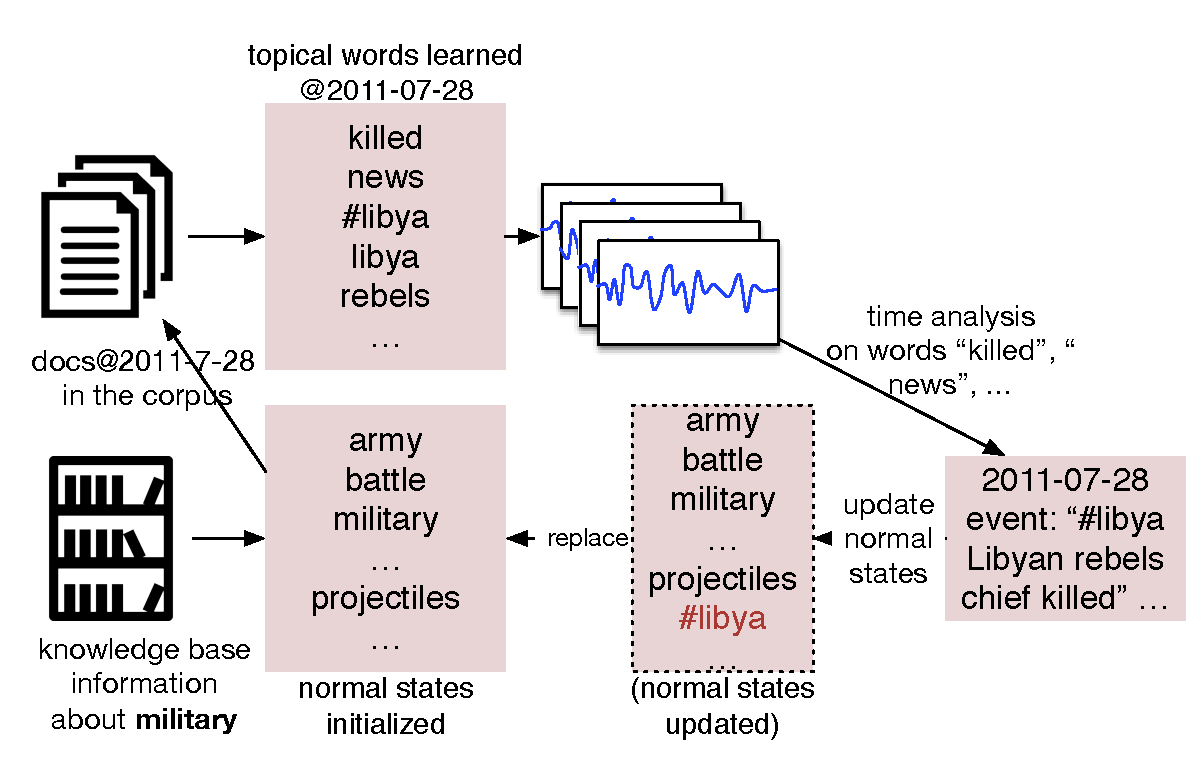
\includegraphics[width=.44\columnwidth]{img/NSDetectorExample.pdf}
                \label{fig:modelDesc}

        }
        \subfigure[Extracting Category-Level Topics in Knowledge Base]{
                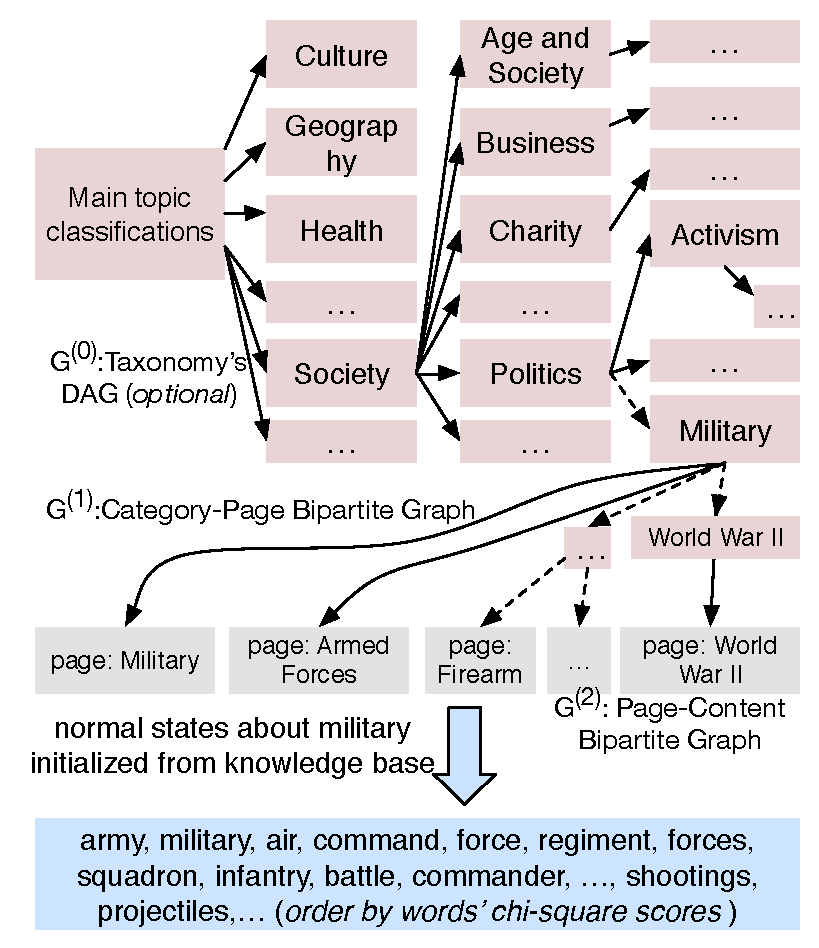
\includegraphics[width=.44\columnwidth]{img/initializationExample.pdf}
                \label{fig:NSinitializaton}
        }
        \caption{(a) \textsc{TransDetector}'s process flow, taking \textit{Military} related events in microblogs as an example. \textsc{TransDetector} includes three phases: extracting category-level topics in knowledge base, conducting transfer learning to get category-level topics in microblog stream, and detecting events from category-level word time series; (b) Illustration on how to extract category-level topics in knowledge base via its three fold hierarchical structure, taking \textit{Military} as an example.}
\end{figure}

To sum up, the contribution of this paper is mainly in four aspects.
(1) We propose a structure-guided category-level topics extraction method, exploiting the knowledge base's hierarchical structure to extract categories' highly correlated topics. 
(2) We develop a probabilistic model CTrans-LDA for category-level transfer learning, which utilizes the word co-occurrences and transfers the knowledge base's category-level topics into microblogs. 
(3) Events are detected accurately on category-level word time series, due to richer semantics and less noise. 
(4) Experiment verifies the quality of category-level topics extracted from knowledge base, and the further study on the benchmark \textit{Edinburgh twitter corpus} validates the effectiveness of our proposed transfer learning method for event detection.

\section{Related Works}
\label{sec:relatedWorks}
\textbf{Event Detection.} Based on how much data are used, the methods are mainly in two groups, the detection \textit{without extra information} and that by \textit{leveraging extra information}. 

Most existing methods are implemented \textit{without extra information}.
They are mainly carried out by clustering articles\cite{Allan:2000wu,Petrovic:2010uj,Wurzer:2015wq}, analyzing word frequencies\cite{Mathioudakis:2010fc,Weng:2011wz}, or finding bursty topics\cite{Diao:2012wj,Yan:2015wm} etc. 
(1) By clustering articles, UMass\cite{Allan:2000wu}, LSH\cite{Petrovic:2010uj}, k-Term-FSD\cite{Wurzer:2015wq} and other similar methods model the occurred events as clusters of articles.
The decision is based on whether the dissimilarity between the incoming article and existed event clusters is over the user-specified threshold. 
(2) By analyzing word frequencies, EDCoW\cite{Weng:2011wz} exploits wavelet transformation, which converts signal from time domain to time-scale domain, to detect the change point of word signal. 
However they treat the word as the most basic unit in analysis, without regarding polysemy words.
(3) By finding bursty topics via topic modelling, TimeUserLDA\cite{Diao:2012wj}, BurstyBTM\cite{Yan:2015wm} generates detected events.
TimeUserLDA distinguishes user's long term interests and short term bursty events, and BurstyBTM utilizes the burstiness of biterms as prior knowledge.
This kind method needs to set the appropriate number of topics, and detects the ``large" events but ignore the ``small" ones. 
To summarize, due to microblog's short length and high noise, it's not easy to set the directly applicable parameter for existing methods to achieve high precision and high recall simultaneously.

The second group methods detect events by \textit{leveraging extra information}. 
\cite{huang2016efficient} incorporates user's and the followees' profiles to help to detect the events of public concern. 
However it's not easy to get this kind contextual information.
\cite{osborne2012bieber} compares two time series generated by event-related tweets and the corresponding Wikipedia article's page views, and further filter out spurious events of microblogs.
Twevent \cite{Twevent2012} divides the tweet into segments according to the Microsoft Web N-Gram service and Wikpedia, then detect the bursty segments and cluster these segments into candidate events for necessary post processings.
But as shown in \cite{Yan:2015wm}, Twevent is still hampered by the performance of simply clustering the bursty segments.
Beyond the scope of microblog stream, \cite{steiner2013mj} utilizes the concurrent wikipedia edit spikes for event detection.
%And \cite{liuleveraging2016} leverages the ACE corpus\cite{doddington2004automatic} and the structure of FrameNet\cite{baker1998berkeley} to improve the event detection within FrameNet, but has not shown how to apply the knowledge base for more general unstructured corpus.
In a nutshell, existing works are different from ours, as we transfer the category information of knowledge base into microblog's words and get the finer processing objects in event detection, rather than treating the knowledge base as a lookup table or a comparison base.

\textbf{Knowledge Base.} Many general knowledge bases and customized knowledge bases are constructed and utilized for different text mining tasks. 
For example, Probase\cite{wu2012probase} constructs a large general probabilistic \textit{IsA} taxomomy from webpages, and is used for semantic web search, and text classification\cite{wang2014concept}.
Such kind efforts are also made by DBPedia\cite{auer2007dbpedia}, Yago\cite{fabian2007yago}, and Freebase\cite{bollacker2008freebase}. 
These works manages knowledge as tuples on graph. 
However the query on large graph is very expensive\cite{huang2011scalable}, which is not very suitable for the scene of quickly and accurately detecting events.

The customized knowledge bases such as EVIN\cite{kuzey2014evin}, Event Registry\cite{leban2014eventRegistry}, and Story-base\cite{wu2015storybase}, are designed for managing events.
These knowledge bases are mainly built on news articles.
EVIN maps the existing event-related news articles into semantic classes. 
Event Registry collects the articles by the API of News Feed Service\cite{trampuvs2012newsfeed}, then detects events, and provides the structural information of the events, such as the related Wikipedia article, timestamp, and location etc. 
Storybase introduces Wikipedia current events\footnote{\url{https://en.wikipedia.org/wiki/Portal:Current_events}} as the resources for constructing event-and-storyline knowledge base on news articles, which are provided by GDELT project\cite{leetaru2013gdelt}.
As the news articles may lag behind the microblogs when the emergency of events, it's not enough to detect events from microblog stream by directly applying these customized knowledge bases. 

\section{\textsc{TransDetector}} 
\label{sec:TransDetector}
In this section, we present a novel category-level transfer learning method for event detection, namely \textsc{TransDetector}. 
Illustrated in Figure \ref{fig:modelDesc}, \textsc{TransDetector} consists of three parts: (1) extracting category-level topics in knowledge base, (2) conducting transfer learning to get category-level topics in microblog stream, and (3) detecting events from category-level word time series.
The following definitions are used by our method \textsc{TransDetector}. 
Definition 1 is used in the \textbf{extracting} phase, Definitions 2 and 3 are used in the \textbf{conducting transfer learning} phase, and Definitions 4 to 6 are used in the \textbf{detecting} phase.
Because Definitions 2 to 6 are very easy to understand, what needs to be specified are Definition 1.
\textit{Category-level topics in knowledge base} is a set of tuples extracted from knowledge base, which weighs the importance of given words to the specific category, defined in Definition 1 formally. 
Taking the \textit{Military} category in Figure \ref{fig:NSinitializaton} as an example, the category-level topic of \textit{military} contain the words \textit{army}, \textit{military}, and \textit{shootings} etc, which are highly related to the category \textit{Military}.

\begin{rmkWithoutSpacing}[\textbf{Category-Level Topics in Knowledge Base}] 
Given category \(c\), the category level topic in knowledge base is defined by a set of tuples, in which the first element is the word \(w^{(c)}_i\) related to the category \(c\), and the second element is the chi-square score \(chi(c,w^{(c)}_{i})\) under the category \(c\). 
And we denote \(c\)'s category-level topic in knowledge base as \(\bm{h}_c=\{<w^{(c)}_i,chi(c,w^{(c)}_{i})>\}_{i=1}^{N_c}\).
\end{rmkWithoutSpacing}

\begin{rmkWithoutSpacing}[\textbf{Category-Level Topics in Microblog Stream}] 
Given category \(c\), the category level topic in microblog stream at time \(t\) is defined by a set of tuples, and denoted as \(\bm{r}_{c,t}=\{<w^{(c)}_i,n(c,t,w^{(c)}_{i})>\}_{i=1}^{N_c}\), in which word \(w^{(c)}_{i}\) is related to the category \(c\), and \(n(c,t,w^{(c)}_{i})\) is its document frequency in the time window \(t\).
\end{rmkWithoutSpacing}

\begin{rmkWithoutSpacing}[\textbf{Category-Level Word Time Series}] 
Given category \(c\) and word \(w\), the category level word time series is a list of document frequencies extracted from \(\{\bm{r}_{c,t}\}_{t=1}^{T}\), and denoted as \(\{n(c,t,w^{(c)}_{i})\}_{t=1}^{T}\).
\end{rmkWithoutSpacing}


\begin{rmkWithoutSpacing}[\textbf{The Set of Events' Candidate Words}] 
The set of events' candidate words \(\mathcal{B}_{c,t}\) are groups of the bursty words in \(\bm{r}_{c,t}\).
\end{rmkWithoutSpacing}

\begin{rmkWithoutSpacing}[\textbf{Event Phrase}] 
Event phrase \(\mathcal{C}_{c,t,i}\) is the \(i\)-th combination of words which occurred in the set of events' candidate words \(\mathcal{B}_{c,t}\), and represents the \(i\)-th event happened in time \(t\) under the category \(c\).
\end{rmkWithoutSpacing}

\begin{rmkWithoutSpacing}[\textbf{Event Related Microblogs}] Event related microblogs \(\mathcal{D}_{c,t,i}\) are articles relating to the \(i\)-th event in time \(t\) of category \(c\), and correspond to the event phase \(\mathcal{C}_{c,t,i}\).
\end{rmkWithoutSpacing}


Section \ref{subsec:hs_initialization} explains the details of how to extract \textit{category-level topics in knowledge base} by using the three fold hierarchical structure.
Section \ref{subsec:rs_initialization} shows how to conduct transfer learning to get \textit{category-level word time series} in microblog stream.
And section \ref{subsec:detection} interprets the high accuracy event detection based on the processed \textit{category-level word time series}.

\subsection{Extracting Category-Level Topics in Knowledge Base}\label{subsec:hs_initialization}
In this part, we discuss in detail how to extract the \textit{category-level topics in knowledge base} on the given categories. 
The knowledge base such as Wikipedia has the structure of classes, subclasses, instances, and the edges between them. 
This structure usually can be represented as triples in RDF graph\cite{klyne2006rdf}, which is adopted to build DBPedia\cite{auer2007dbpedia} and YAGO\cite{suchanek2007yago} from Wikipedia. 
But the the query on the large graph is usually very expensive\cite{huang2011scalable}. 
To make a trade-off between cost and performance, we use the lightweight data structure \textit{topics} to represent the knowledge at category(class) level.
And the knowledge base's threefold structure \(G^{(0)}\), \(G^{(1)}\), \(G^{(2)}\) benefits the extraction of \textit{category-level topics}. 

\textbf{Taxonomy Graph \(G^{(0)}\)}. The directed edges in \(G^{(0)}\) represent the \textit{class}\(\rightarrow\)\textit{subclass} relations in the knowledge base. 
Taking Wikipedia for example (Figure \ref{fig:NSinitializaton}), the node \textit{Main topic classifications}\footnote{\url{https://en.wikipedia.org/wiki/Category:Main_topic_classifications}} has the subclass \textit{Society}, further contains the subclass \textit{Politics}, which is the ancestor of the subclass \textit{Military}.
As \(G^{(0)}\) is not a Directed Acyclic Graph originally\cite{faralli2015large}, we remove the cycles according to nodes' PageRank-HITS\cite{Yan:2015wq} score.
Specifically, the edges \textit{class}\(\rightarrow\)\textit{subclass} are preserved only when the node \textit{class} has the higher PageRank-HITS score than the node \textit{subclass}, which is shown in the line \ref{alg:line2inNormalStatesInit} of Algorithm \ref{alg:normalStatesInit}.
After removing cycles, the taxonomy structure on the knowledge base is better represented by the directed acyclic graph \(G^{(0)'}\).
As shown in line \ref{alg:line3inNormalStatesInit} of Algorithm \ref{alg:normalStatesInit}, by visiting the category \textit{Military} in the DAG \(G^{(0)'}\), the breadth-first traverse can reach its successor sub-category nodes such as \textit{Firearms}, \textit{The World Wars}, and \textit{World War II}, etc. 

\textbf{Category-Page Bipartite Graph \(G^{(1)}\)}. 
The directed edges in \(G^{(1)}\) represent the \textit{class}\(\rightarrow\)\textit{instance} relations in the knowledge base.
In Wikipedia, by considering \(G^{(0)'}\) and \(G^{(1)}\) together as shown in line \ref{alg:line5inNormalStatesInit} of Algorithm \ref{alg:normalStatesInit}, we can get all the pages related to the given category. 

\textbf{Page-Content Map \(G^{(2)}\)}. 
For a specific Wikipedia dumps version, the edges  \textit{page} \(\rightarrow\)\textit{content} in \(G^{(2)}\) define a one-to-one mapping.
There are a bulk of information stored in the wiki text content.
In order to extract the key words in wiki page's content, which distinguish it from other pages, we use the chi-square statistics\cite{yang1997comparative}\cite{liu2009imbalanced} to measure the importance of each word for the specific page.

For a given category in \(G^{(0)'}\), chi-square statistics also can evaluate the importance of each word appeared in text contents. 
For example, the chi-square statistic of the term \textit{shooting} under the category \textit{military} is 2888.7 under chi-square test with 1 degree of freedom.
That means the term \textit{shooting} is highly related to the category \textit{military}.  
%To prevent the overclaim of rare word by chi-square statitistcs, the word frequency is introduced as a supplement\cite{liu2009imbalanced}, as shown in line \ref{alg:line10inNormalStatesInit} of Algorithm \ref{alg:normalStatesInit}.
Finally, we can get the \textit{category-level topic}, which are  composed by the category related words and their corresponding importance.
\setlength{\textfloatsep}{3pt}% Remove \textfloatsep
\begin{algorithm}[h]
\scriptsize
\caption{Extraction of Category-Level Topics in Knowledge Base}
\label{alg:normalStatesInit}

\KwIn{Taxonomy's Graph \(G^{(0)}\), Category-Page Bipartite Graph \(G^{(1)}\), Page-Content Bipartite Graph \(G^{(2)}\), topic related category node \(c\)}
\KwOut{\(c\)'s category-level topic in knowledge base \(\bm{h}_c\)}
\(Pages(c)\leftarrow \varnothing\), \(\bm{h}_c \leftarrow \varnothing\)\\
DAG \(G^{(0)'} \leftarrow\) Remove Cycles of \(G^{(0)}\) by nodes' HITS-PageRank scores. \label{alg:line2inNormalStatesInit}\\
\(SuccessorNodes(c) \leftarrow \) Breadth-first-traverse(\(G^{(0)'},c\))\label{alg:line3inNormalStatesInit}\\
\For{\(node \in SuccessorNodes(c)\)}{
    \(Pages(c) \leftarrow Pages(c) \cup G^{(1)}.neighbours(node)\) \label{alg:line5inNormalStatesInit}\\
}
Word frequency table \(n(c,.) \leftarrow \) do word count on the text contents of \(Pages(c)\) \\
Word frequency table \(n(All,.) \leftarrow \) do word count on the text contents of all pages in \(G^{(2)}\).\\
\For{word \(w\) in WordFrequencyTable(All).keys()}{
    \(chi(c,w) \leftarrow \) \(w\)'s chi-square statistics on \(WordFrequencyTable(c)\) and \(WordFrequencyTable(All)\).\\
    \(h_{c,w} \leftarrow chi(c,w)\) \label{alg:line10inNormalStatesInit}\\
}
\Return{\(\bm{h}_c\)}
\end{algorithm}

Considering the full Wikipedia's contents, the word's score in the \textit{category-level topic} evaluates the importance of word to the concerned category accurately. 
For example, in \textit{Military}'s \textit{category-level topic}, the top  words are \textit{army}, \textit{military}, \textit{air}, \textit{command}, \textit{force}, and \textit{regiment}, etc. 
The document which contains these words is related to the category \textit{Military} with high probability. 

\subsection{Conducting Transfer Learning}
\label{subsec:rs_initialization}
In this subsection, we describe how the proposed probabilistic model CTrans-LDA transfers the category-level topics into microblogs.

There are two facts inspiring CTrans-LDA. 
(1) The topics in the document may contain category-level topics. 
As an example, the tweet ``Libyan rebel chief gunned down in Benghazi (2011-07-28)'' contains the topic that is similar to the \textit{Military}'s \textit{category-level topics in knowledge base}.
(2) The \textit{category-level topics in microblog stream} can reuse the information stored in the corresponding \textit{category-level topics in knowledge base}.
The word \textit{libyan} in the aforementioned example tweet ranks much higher in the \textit{Military} and the \textit{Middle East} category-level topics than the other categories' topics.
After considering the relatedness between the remaining context and the \textit{category-level topics in knowledge base}, the learned topics of the example tweet include \textit{Military} and \textit{Middle East}. 

The generative process of CTrans-LDA can be described as follows.
\begin{enumerate}[topsep=0pt,itemsep=0mm]
\item Draw corpus prior distribution \(\bm{m} \sim Dir(\alpha \bm{u})\), where \(\bm{u}\) is the uniform distribution.
\item For each topic \(k \in \{1,\cdots,K\}\), 
\begin{enumerate}[itemsep=0mm]
\item word distribution on the topic \(\bm{\phi_k} \sim Dir(\bm{\beta}+ \bm{\tau_k})\).
\end{enumerate}
\item For each document index \(d \in \{1,\cdots,D\}\),
\begin{enumerate}[itemsep=0mm]
\item topic distribution on the document \(\theta_d \sim Dir(\bm{m})\),
\item for each word index \(n \in \{1,\cdots,N_d\}\),
\begin{enumerate}[itemsep=0mm]
\item word's topic assignment \(z_{dn} \sim Multinomial(\theta_d)\), 
\item word \(w_{dn} \sim Multinomial(\phi_{z_{dn}})\). 
\end{enumerate}
\end{enumerate}

\end{enumerate}

In the above generative process, the line 2(a) is the key point to distinguish CTrans-LDA from LDA\cite{blei2003latent}, where \(\bm{\tau}_k\) is defined by Equation(\ref{eq:wikiPrior}).
\(K_{KB}\) is the number of pre-defined categories used for transferring, and \(S_k\) is the set of words appeared in the \(k\)-th category-level topic.
As \cite{wallach2008structured} mentioned that the asymmetric prior distribution can significantly improve the quality of topic modelling, \(\bm{\phi_k} \sim Dir(\bm{\beta}+ \bm{\tau_k})\) incorporates \textit{category-level topics in knowledge base} into the asymmetric prior of the word distribution on topic. 
The effect of \(\bm{\tau_k}\) is obvious, e.g., \(\tau_{Military,army}/\tau_{Military,basketball}=203\) leads to that topic \textit{Military} prefers to contain the word \textit{army} other than \textit{basketball}.
The parameter \(\lambda\) controls how much the knowledge is used for transferring, which can be chosen by cross-validated grid-search. 

\setlength{\abovedisplayskip}{0pt}
\setlength{\belowdisplayskip}{0pt}
\begin{scriptsize}
\begin{equation}
\label{eq:wikiPrior}
\begin{aligned}
\tau_{kv}=
\left\{ \begin{aligned}
\lambda \frac{h_{kv}}{\sum_{v\in S_{k}}h_{kv}} &,v\in S_{k}\ and  \ k \leq K_{\bm{KB}} \\
0&,v \notin S_{k} \ or \ k > K_{\bm{KB}} \\
\end{aligned}\right.
\end{aligned}
\end{equation}
\end{scriptsize}

To solve CTrans-LDA, the gibbs sampling is adopted to determine the hidden variable \(z_{dn}\) and the model parameter \(\phi_k\).
In the initialization phase of Gibbs sampling for CTrans-LDA, the hidden variable \(z_{dn}\) is initialized to topic \(k\) with probability \(\hat{q}_{k|v}\) as Equation (\ref{eq:initProbability}).
For the word \(v\) that belongs to any category-level topic, \(\hat{q}_{k|v}\) is proportional to its importance in the category-level topic \(\tau_{kv}\) as Equation \ref{eq:initProbability}(a). 
For the new word \(v\) in text stream, \(\hat{q}_{k|v}\) is   set uniformly \(1/(K-K_{\bm{KB}})\) on the other topics as Equation \ref{eq:initProbability}(b,c). 
The initialization makes sure that the learned topics are aligned to the pre-defined category-level topic.
\setlength{\abovedisplayskip}{0pt}
\setlength{\belowdisplayskip}{0pt}
\begin{scriptsize} 
\begin{equation}
\label{eq:initProbability}
\begin{aligned}
\hat{q}_{k|v}=
\left\{ \begin{aligned}
\frac{\tau_{kv}}{\sum_{k=1}^{K}\tau_{kv}} &,\sum_{k}\tau_{kv}>0 & (a)\\
0&, \sum_{k}\tau_{kv}=0 \ and \ k \leq K_{\bm{KB}} & (b)\\
1/(K-K_{\bm{KB}})&,\sum_{k}\tau_{kv}=0 \ and \ k > K_{\bm{KB}} & (c)
\end{aligned}\right.
\end{aligned}
\end{equation}
\end{scriptsize}

%采样公式p(z|.),z有两部分。
The sampling process uses the conditional probability \(p(z_{dn}=k|.)\propto (n^{(d)}_{dk}+\alpha m_k)(n^{(w)}_{kv}+\tau_{kv}+\beta)/(n^{(w)}_{k,.}+\tau_{k,.}+V\beta)\), where \(n^{(d)}_{dk}\) is the number of words in document \(d\) assigned to topic \(k\), and \(n^{(w)}_{kv}\) is the times of word \(v\) assigned to topic \(k\).
We set \(\alpha=0.1\) and \(\beta=0.005\) according to the suggestion by \cite{tang2014understanding}.


After Gibbs sampling on discrete time windows, CTrans-LDA learned all hidden topics of words in microblog stream.
And for a specific word type \(w\) and its category assignment \(c\) in time window \(t\), its document frequency is counted as \(n(c,t,w^{(c)})\), which is the element of category-level word time series.
Event detection on category-level word time series is discussed in the following subsection.

\subsection{Detecting Events from Category-Level Word Time Series}
\label{subsec:detection}
After transfer learning, it's much easier to detect the event from category-level word time series, which is shown in Figure \ref{fig:hood}. We take the detection in three sub-phases: (1) detecting events' candidate words; (2) generating event phrases; and (3) retrieving event related microblogs.
Note that these sub-phases are also available for the common text stream, but they performs better when words are enriched by category concepts of knowledge base.
%这里添加对这几个Definition的解释。

\textbf{Detecting events' candidate words}. For a word \(w\) and a category \(c\), on its time series \(\{n(c,t,w^{(c)})\}_{t=1}^{T}\), many bursty detection methods can be applied to check if the word \(w\) is bursty in category \(c\) by given time \(t\). 
In our paper, we assume the document frequency of \(w^{(c)}\) follows a poisson distribution, which is also used in \cite{Diao:2012wj}.
And the document frequency of nonbursting \(w^{(c)}\) has the possison distribution with the parameter \(\lambda=\mu_0\); while the bursting one with the parameter \(4\mu_0\) means the document frequency \(n(c,t,w^{(c)})\) is much higher when bursting.
We empirically set \(\mu_0\) as the moving average \(\mu_0^{(t)}=\frac{1}{T}\sum_{\tau=t-T}^{t-1}n(c,\tau,w^{(c)})\), and set T=10.
Hence, at time \(t\), bursty or not is determined by comparing the probabilities of above poisson distributions. 
After bursty detection on the time series, we add each time \(t\)'s bursty word \(w^{(c)}\) into the set of event's candidate words \(\mathcal{B}_{c,t}\).

\textbf{Generating event phrases}. 
In the set of event's candidate words \(\mathcal{B}_{c,t}\), some words appear together and should be grouped into event phrases.
For example, there are six bursty words in \(\mathcal{B}_{military,2011-07-28}\) belonging to two event phrases \textit{``ft, hood, attack"} and \textit{``libyan, rebel, gunned"} in the time window 2011-07-28 to represent the events happened to the US military establishment and the Libyan rebel respectively. 

To group the bursty words together, we  construct the directed weighted graph \(\mathcal{G}_{c,t}=(\mathcal{B}_{c,t},\mathcal{E}_{c,t},\mathcal{W}_{c,t})\), where \(\mathcal{E}_{c,t}=\{(a,b)|a \in \mathcal{B}_{c,t}, b \in \mathcal{B}_{c,t}, PMI(a,b)>0 \}\), and \(\mathcal{W}_{c,t}\) gives the PMI scores on the edges.
The graph \(\mathcal{G}_{c,t}\) means the words in \(\mathcal{B}_{c,t}\) are connected if and only if their PMI score in the given time window's microblogs is over 0. 
Given the graph \(\mathcal{G}_{c,t}\), the spectral clustering\cite{von2007tutorial} is utilized for exploring the best partition of words. 
To get the optimum cluster number, we use the graph density as the criteria.
The graph density is the ratio of the number of edges to that of complete graph (the graph with all possible edges). 
We search the best cluster number from 1 to \(|\mathcal{B}_{c,t}|\), and stop when all the resulting sub-graphs satisfy the criteria that the density is over the threshold, which is set to 0.6 empirically.
In this way, the generated event phrase combines the co-occurred bursty words and excludes the unrelated. 


\textbf{Retrieving event related microblogs}. 
To better understand the event, we retrieve the event microblogs \(\mathcal{D}_{c,t,i}\) by using the event phrase \(\mathcal{C}_{c,t,i}\).
Generally, according to the number of bursting words in the event phrase \(\mathcal{C}_{c,t,i}\), there are two situations to be addressed. 
(1) \(|\mathcal{C}_{c,t,i}|=1\), we directly add the microblog in time window \(t\), which contains the bursting category-word \(w^{(c)}\), into the set \(\mathcal{D}_{c,t,i}\).
(2) \(|\mathcal{C}_{c,t,i}|\geq 2\), it's not necessary that all the bursting words are included in the event related microblog.
For example, the tweet ``\textit{Soldier wanted to attack Fort Hood troops}" contains the bursting words \textit{attack} and \textit{hood}, not all the event phrase ``\textit{ft, hood, attack}". 
To tackle this problem, we consider the microblog, that contains any pair of category-words in the event phrase, as the event related microblog. 
Finally, \textsc{TransDetector} gets the detected events \(\{(\mathcal{C}_{c,t,i},\mathcal{D}_{c,t,i})\}_{i=1}^{|\mathcal{C}_{c,t}|}\), containing the event phrase and the corresponding event related microblogs for the given category and the time window.

%Text stream evolves more quickly with time than knowledge base.
%For example, recent state of Military contain .





\section{Experiments}
%\subsection{Data Sets}
In this subsection, we demonstrate the effectiveness of \textsc{TransDetector}, by evaluating the \textit{category-level topics in knowledge base}, \textit{category-level topics in microblog stream} learned by transfer learning, and the effect of event detection. 

\textbf{Knowledge Base.} 
We construct the taxonomy graph \(G^{(0)}\), the category-page bipartite graph \(G^{(1)}\) from the latest dump of category links\footnote{\url{https://dumps.wikimedia.org/enwiki/latest/enwiki-latest-categorylinks.sql.gz}} and the page-content map \(G^{(2)}\) from Wikipedia pages\footnote{\url{https://dumps.wikimedia.org/enwiki/latest/enwiki-latest-pages-articles.xml.bz2 }}.
We set \(K_{KB}=50\), which means 50 categories are selected manually to cover the topics of Wikipedia and the target corpus as widely as possible. 
There are two kinds of categories are considered. 
The mid-high categories in the taxonomy graph \(G^{(0)'}\), which are representative, are likely to be selected, such as \textit{Aviation}, \textit{Military}, and \textit{Middle East}, etc.
And the mid categories, which reflect the main interests of the target corpus, are also taken into consideration, such as \textit{American Football}, \textit{Basketball}, and \textit{Baseball}, etc. 
%Other knowledge bases which have the above mentioned threefold structure are also available for conducting.

\textbf{Microblog Stream Dataset.} We conduct the empirical analysis on a text stream benchmark \textit{Edinburgh twitter corpus} which is constructed by \cite{petrovic2012using} and widely used by previous event detection researches \cite{petrovic2013can} \cite{Wurzer:2015wq}. 
Due to the developer policy of Twitter, \cite{petrovic2012using} only redistributes tweets' IDs\footnote{\url{http://demeter.inf.ed.ac.uk/cross/docs/fsd_corpus.tar.gz}}.
%\footnote{\url{https://dev.twitter.com/overview/terms/policy}}
We collected the tweets' contents according to the IDs with the help of Twitter API. 
Though we cannot get the whole dataset due to the limit of Twitter API, after necessary pre-processing, our rebuilt dataset still contains 36,627,434 tweets, which also spans from 2011/06/30 to 2011/09/15.
More details of the original dataset are described in \cite{petrovic2010edinburgh}.

\subsection{Evaluation on Categroy-Level Topics in Knowledge Base}
The category-level topics are initialized on the pre-defined categories from the knowledge base as Algorithm \ref{alg:normalStatesInit}.

\textbf{Evaluation Metrics.}
We compare the topic coherence of category-level topics with the topics learned from Wikipedia by LightLDA\cite{yuan2015lightlda} in terms of NPMI\cite{Rder2015ExploringTS}.
Different from traditional experiments that only compute the topic coherence of top words, we want to check whether  it can hold for more words.
Due to the limit of NPMI computing module\footnote{\url{https://github.com/AKSW/Palmetto}}, which computes the coherence of up to 10 words each time, we compute NPMI on the combination of top five words with each next five words as Table \ref{tbl:NPMIDetails}.

\textbf{Results.}
Observe that even for the combination of 96th to 100th words with the top five words in \textit{Aviation}'s category-level topics in knowledge base, NPMI=0.131 shows that the topic coherence still holds well without drifting.
More generally, Figure \ref{fig:NPMI} illustrates that the category-level topics are much more stable than the topics learned by LightLDA.
Taking the group 10 (the combination of 56th to 60th words with the top five words) as an example, the median one of category-level topic performs better than those learned by LightLDA. 
And more topics are compared shown in Figure \ref{fig:NPMI}, proving that our method performs better at extracting key features for categories.

\begin{table}[h]
\setlength{\abovecaptionskip}{0.cm}%set the distance between caption and table to 0 cm.
\setlength{\belowcaptionskip}{0.cm}
\centering
\caption{The comparison on the topic coherence(NPMI) between our method and LightLDA\cite{yuan2015lightlda}, taking \textit{Aviation} as an example. (GID is short for Group Id. * means each group contains the five top words. NPMI is computed on a group of ten words. \(\sim\) stands for the top five words.)}
\scalebox{0.65}{
\begin{tabular}{|c|l|l|c !{\vrule width 1pt} c|l|l|c|}
\hline
\multicolumn{4}{|c!{\vrule width 1pt}}{Category-Level Topics extracted from Wikipedia by \textsc{TransDetector}} & \multicolumn{4}{c|}{Topics Learned from Wikipedia by LightLDA\cite{yuan2015lightlda}}    \\ \hline
GID& \#words*  & words  & NPMI & GID& \#words*& words & NPMI \\ \hline
- & 1-5 & aircraft air airport flight airline &-& - & 1-5 & engine aircraft car air power &-\\ \hline
0 & 1-5, 6-10 & \(\sim\), airlines aviation flying pilot squadron &  0.113 & 0 & 1-5, 6-10 & \(\sim\), design flight model production speed & 0.112\\ \hline
1 & 1-5, 11-15 & \(\sim\), flights pilots raf airways fighter & 0.155 & 1 & 1-5, 11-15 &\(\sim\), system vehicle cars engines mm & 0.062\\ \hline
2 & 1-5, 16-20 & \(\sim\), boeing runway force crashed flew   & 0.092 & 2 & 1-5, 16-20 & \(\sim\), fuel vehicles designed models type & 0.072\\ \hline
3 & 1-5, 21-25 &\(\sim\), airfield landing passengers plane aerial & 0.179 & 3 & 1-5, 21-25 & \(\sim\), version front produced rear electric & 0.035\\ \hline
4 & 1-5, 26-30 &\(\sim\), bomber radar wing bombers crash & 0.137 & 4 & 1-5, 26-30 & \(\sim\), space control motor standard development & 0.085\\ \hline
5 & 1-5, 31-35 &\(\sim\), airbus airports operations jet helicopter & 0.189 & 5 & 1-5, 31-35 & \(\sim\), film range light using available & -0.002\\ \hline
6 & 1-5, 36-40 &\(\sim\), squadrons base flown havilland crew & 0.088 & 6 & 1-5, 36-40 & \(\sim\), wing powered wheel weight launch & 0.087\\ \hline
7 & 1-5, 41-45 & \(\sim\), combat luftwaffe aerodrome carrier fokker & 0.159 & 7 & 1-5, 41-45 & \(\sim\), developed low test ford cylinder & 0.007\\ \hline
8 & 1-5, 46-50 &\(\sim\), planes fly engine takeoff fleet & 0.186 & 8 & 1-5, 46-50 & \(\sim\), equipment side pilot hp aviation & 0.091\\ \hline
9 & 1-5, 51-55 &\(\sim\), fuselage helicopters aviator naval aero & 0.157 & 9 & 1-5, 51-55 & \(\sim\), systems us sold body drive & -0.051\\ \hline
10 & 1-5, 56-60 &\(\sim\), glider command training balloon faa & 0.166 & 10 & 1-5, 56-60 & \(\sim\), gear introduced class safety seat & 0.069\\ \hline
\(\cdots\) & \(\cdots\) &\(\cdots\) &\(\cdots\) & \(\cdots\) & \(\cdots\) &\(\cdots\) &\(\cdots\)\\ \hline
18 & 1-5, 96-100 &\(\sim\), scheduled carriers military curtiss biplane &0.131 & 18 & 1-5, 96-100 & \(\sim\), transmission special replaced limited different & 0.059\\ \hline
19 & 1-5, 101-105 &\(\sim\), accident engines iaf albatross rcaf &0.068 & 19 & 1-5, 101-105 & \(\sim\), features machine nuclear even unit & 0.011\\ \hline
\end{tabular}
}
\label{tbl:NPMIDetails}
\end{table}

\begin{figure}[h]
	\setlength{\abovecaptionskip}{0.cm}
	\setlength{\belowcaptionskip}{0.cm}
        \centering
        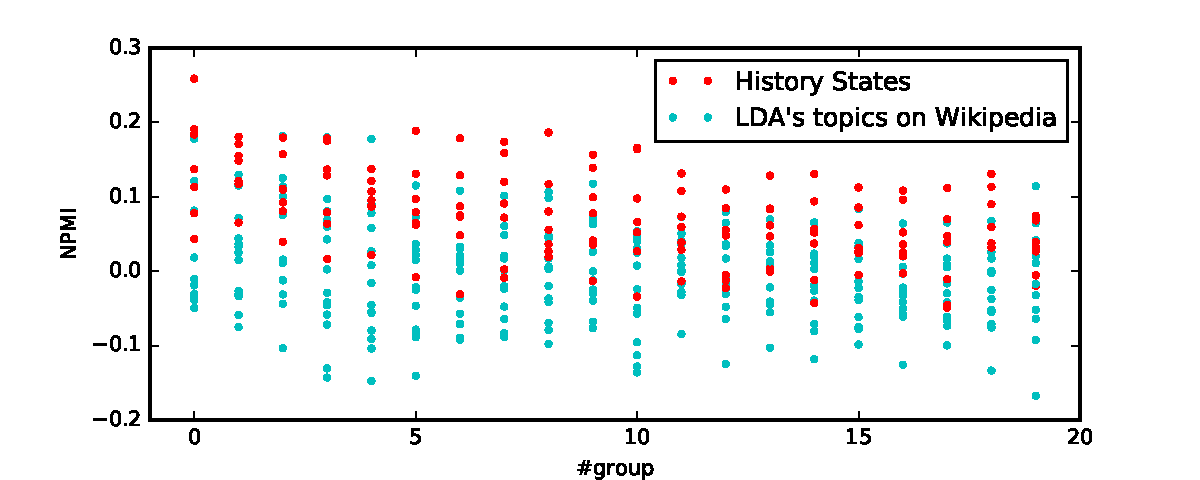
\includegraphics[width=1.0\columnwidth]{img/NPMI.pdf}
        \caption{More topics are compared at the NPMI metrics between our method and LightLDA}
        \label{fig:NPMI}
\end{figure}

For CTrans-LDA, \(K\) is set to be 200, which means CTrans-LDA learned 50 category-level topics and 150 other topics.
After cross-validated grid-search, \(\lambda\) is set to be 12.8. The other parameters are set as \(\alpha=0.1\), \(\beta=0.005\).
We run CTrans-LDA window by window on text stream, and learn specific categories' topics.
The result in Table 2 demonstrates the effectiveness of transferring category-level topics into the microblog stream, and finding more new words in the stream which is not stored in the knowledge base.


\begin{table*}[ht]
\setlength{\abovecaptionskip}{0.cm}%set the distance between caption and table to 0 cm.
\setlength{\belowcaptionskip}{0.cm}
\centering
\caption{Category-Level Topics extracted from knowledge base and the corresponding topics on microblog stream learned from CTrans-LDA, taking the categories \textit{Aviation},  \textit{Health}, \textit{Middle East}, \textit{Military}, and \textit{Mobile Phones} as examples. The words in \textbf{\textit{bold italic}} font are newly learned on the microblog stream by the transfer learning, which semantic meanings are verified consistent with the categories; while the words in normal font play the role as the bridge in transfer learning, and appear in the both category-level topics in two domains.}
\scalebox{0.8}{
\begin{tabular}{|cc|cc|cc|cc|cc|cc|}
\hline
\multicolumn{2}{|c|}{\textit{Aviation}} & \multicolumn{2}{c|}{\textit{Health}} & \multicolumn{2}{c|}{\textit{Middle East}} & \multicolumn{2}{c|}{\textit{Military}} & \multicolumn{2}{c|}{\textit{Mobile Phones}}\\
\begin{tabular}[c]{@{}c@{}}Knowledge\\ Base\end{tabular} & \begin{tabular}[c]{@{}c@{}}Microblog\\ Stream\end{tabular} & \begin{tabular}[c]{@{}c@{}}Knowledge\\ Base\end{tabular} & \begin{tabular}[c]{@{}c@{}}Microblog\\ Stream\end{tabular} & \begin{tabular}[c]{@{}c@{}}Knowledge\\ Base\end{tabular} & \begin{tabular}[c]{@{}c@{}}Microblog\\ Stream\end{tabular} & \begin{tabular}[c]{@{}c@{}}Knowledge\\ Base\end{tabular} & \begin{tabular}[c]{@{}c@{}}Microblog\\ Stream\end{tabular} & \begin{tabular}[c]{@{}c@{}}Knowledge\\ Base\end{tabular} & \begin{tabular}[c]{@{}c@{}}Microblog\\ Stream\end{tabular} \\ 
\hline
aircraft & air & health & weight & al & \textbf{\textit{\#syria}} & army & killed & android & iphone\\ 
air & plane & patients & loss & israel & \textbf{\textit{\#bahrain}} & military & news & mobile & apple \\ 
airport & flight & medical & diet & iran & people & air & \textbf{\textit{\#libya}} & nokia & android \\ 
flight & time & disease & health & arab & israel & command & libya & ios & app \\
airline & airlines & treatment & cancer & israeli & police & force & rebels & phone & ipad \\
airlines & news & hospital & lose & egypt & \textbf{\textit{\#libya}} & regiment & people & samsung & samsung \\
aviation & boat & patient & fat & egyptian & \#egypt & forces & police & game & mobile\\
flying & airport & clinical & tips & ibn & news & squadron & war & app & blackberry \\
pilot & force & symptoms & treatment & jerusalem & \textbf{\textit{\#israel}} & infantry & libyan & iphone & tablet \\
squadron & fly & cancer & body & syria & world & battle & attack & htc & apps\\
\hline
\end{tabular}
}
\label{tbl:historyStates}
\end{table*}

\subsection{Effects of Event Detection}
\textbf{Baselines Methods.} We compare our proposed method against the following methods, Twevent\cite{Twevent2012}, BurstyBTM\cite{Yan:2015wm}, LSH\cite{Petrovic:2010uj}, EDCoW\cite{Weng:2011wz}, and TimeUserLDA\cite{Diao:2012wj}, which are mentioned in the Section \ref{sec:relatedWorks}.
We implement these competing methods based on the open source community versions, e.g. EDCoW\footnote{\url{https://github.com/Falitokiniaina/EDCoW}}, or the authors' releases, e.g. BurstyBTM\footnote{\url{https://github.com/xiaohuiyan/BurstyBTM}}.
The above methods are set carefully according to the descriptions in the papers.
More precisely, (1) for LSH, 13 bits per hash table, 20 hash tables are set, and top 500 clusters with high entropy are selected as the event candidates; (2) for Twevent, the number of candidate bursty segments is set to be the square root of the window size, the newsworthiness threshold is set to be 4, and 375 candidate events are detected; (3) for EDCoW, the tunable parameter \(\gamma\) value is set to be 40, and 349 bursty ``phrases" are found for evaluation; (4) for TimeUserLDA, the topic number is set to be 500, and the most 100 bursty topics are selected as candidate events; (5) for BurstyBTM, the topic number is set to be 200, which is also the number of bursty topics in the model.
The information about the number of events to be evaluated is listed in Table \ref{tbl:overall}, where TransDetector detects 457 events after filtering out too niche events that contain less than 20 tweets. 

\textbf{Benchmarks and Evaluation Metrics.} 
The evaluation is conducted on two benchmarks.
The first benchmark on \textit{Edinburgh twitter corpus} contains 27 manually labeled events\cite{petrovic2013can}\footnote{\url{http://demeter.inf.ed.ac.uk/cross/docs/Newswire_Events.tar.gz}}, which all exist in our rebuilt dataset on the \textit{Edinburgh twitter}'s IDs.
These labeled events focus on the events that are both mentioned in twitter and newswire,e.g. \textit{``Oslo Attacks"} and \textit{``US Increasing Debt Ceiling"}, but still miss many important events such as \textit{``Hurricane Irene"}, \textit{``Al-Qaida's No. 2 Leader Being Killed"}, and popular events such as \textit{``Harry Potter and the Deathly Hallows (Part 2)"}.
To include these important events and enlarge the ground truth of realistic events pool, we build the second benchmark carefully.
We manually evaluate the candidate events detected by LSH,  \textsc{TransDetector}, Twevent, EDCoW, BurstyBTM, and TimeUserLDA, with the help of the \textit{Wikipedia Current Event Portal}\footnote{\url{https://en.wikipedia.org/wiki/Portal:Current_events}} and a local search engine built on Lucene.
The labeling process generates the Benchmark2, and contains 395 events.
We use precision and recall to evaluate each method on both benchmarks, and utilize the DERate(Duplicate Event Rate) metric\cite{Twevent2012} to measure the readability of detected events.
The smaller the metric DERate, the less duplicate events to be filtered out in the application.


\textbf{Results.}
In general, our method is better than the existing methods in terms of the precision and the recall, only sacrificing in the DERate slightly, as shown in Table \ref{tbl:overall}. 
This is because an event could be grouped into multiple categories (e.g. the event \textit{``S\&P downgrade US credit rating"}, related to the politics category and the financial category simultaneously), but is not a problem as the method \textsc{TrasnDetector} has already achieved the high precision and recall. 

Comparing to \textsc{TrasnDetector}, the existing methods are suffered from having to choose between precision and recall, but not both. 
Taking the method Twevent as an example, which also utilizes the knowledge base for promoting the event detection performance, it has three parameters to trade off, in which the newsworthiness is the most impact one. 
In our experiment, when setting newsworthiness to be 4, Twevent achieves its best performance in terms of F value; lower or higher of value sacrifices the recall or precision. 
The other methods also meet the same problem of tuning parameters, such as the topic number for TimeUserLDA and BurstyBTM, and the distance threshold for LSH.

\begin{table}[h]
\setlength{\abovecaptionskip}{0.cm}%set the distance between caption and table to 0 cm.
\setlength{\belowcaptionskip}{0.cm}
\centering
\caption{Overall Performance on Event Detection}

\scriptsize
\scalebox{1}{
\begin{threeparttable}  

\begin{tabular}{|c|c|c|c|c|c|c|}
    \hline
    Method & \begin{tabular}[c]{@{}c@{}}Number of\\Events to \\ be Evaluated \end{tabular} & \begin{tabular}[c]{@{}c@{}}Recall@ \\ Benchmark1\end{tabular}& \begin{tabular}[c]{@{}c@{}}Precision@ \\ Benchmark2\end{tabular} & \begin{tabular}[c]{@{}c@{}}Recall@ \\ Benchmark2\end{tabular} & \begin{tabular}[c]{@{}c@{}}F@ \\ Benchmark2\end{tabular} & \begin{tabular}[c]{@{}c@{}}DERate\tnote{a}\ \ (Duplicate\\ Event Rate)@\\ Benchmark2\end{tabular} \\ \hline
    LSH & 500 & 0.704 & 0.788 & 0.651 & 0.713 & 0.348 \\ \hline
    TimeUserLDA & 100 & 0.370 & 0.790 & 0.177 & 0.289 & 0.114 \\ \hline
    Twevent & 375 &  0.741 & 0.808 & 0.658 & 0.725 & 0.142 \\ \hline
    EDCoW & 349 & 0.556 & 0.748 & 0.511 & 0.607 & 0.226 \\ \hline
    BurstyBTM & 200 & 0.667 & 0.825 & 0.384 & 0.497 & \textbf{0.079} \\ \hline
    \textsc{TransDetector} & 457 & \textbf{0.889} & \textbf{0.912} & \textbf{0.876} & \textbf{0.894} & 0.170 \\ \hline
    \end{tabular}

\begin{tablenotes}  
\item[a] DERate = (the number of duplicate events) / (the total number of detected realistic events)\cite{Twevent2012}
\end{tablenotes}  
\end{threeparttable}  
}
\label{tbl:overall}
\end{table}

In order to understand why the existing methods cannot perform well, we dive into the results on the Benchmark1, and show the relation between the recall and the event size (number of microblogs related to the events) in Figure \ref{fig:Benchmark1}. 
The 27 events are divided into 4 groups according to its size. 
The first group contains 5 very popular events, having more than 200 microblogs, such as \textit{``S\&P downgrade US credit rating''} with 656 microblogs, \textit{``Atlantis shuttle lands''} with 595 microblogs, etc.
The remaining groups' sizes are listed in the x-axis of Figure \ref{fig:Benchmark1}.
The fourth group contains 11 not-so-popular events, each containing less than 50 microblogs, such as \textit{``War criminal Goran hadzic arrested"} with only 27 microblogs reported.
In our experimental settings, the methods all perform well on the very popular events, but perform worse on the not-so-popular events.
For the not-so-popular events, the underlying bursty pattern is not so obvious that leads many methods to fail to catch the pattern.
We further find out that the number of microblogs in an event follows a power-law distribution, which similar phenomenon is also reported in \cite{Twevent2012}.
The widespread existence of such not-so-popular events challenge almost all the existing event detection methods.
More result in Table 4 shows the examples of military related events detected by \textsc{TransDetector} on the real dataset.

\begin{figure}[h]
	\setlength{\abovecaptionskip}{0.cm}
	\setlength{\belowcaptionskip}{0.cm}
        \centering
        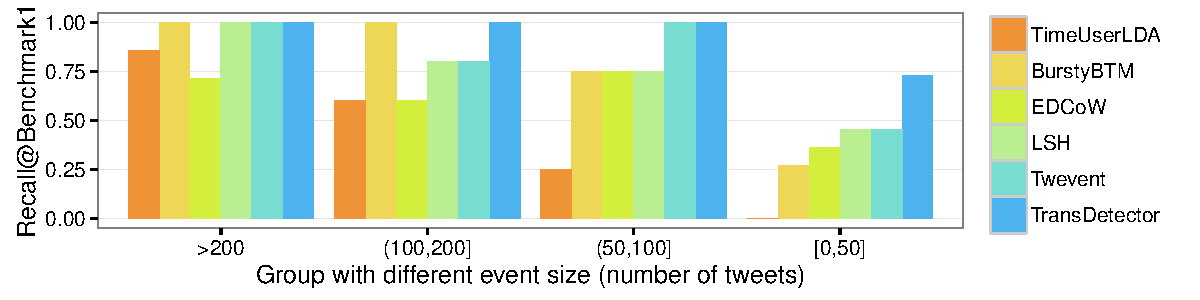
\includegraphics[width=1.0\columnwidth]{img/barchartOnBenchmark1.pdf}
        \caption{The relation between the recall and the event size}
        \label{fig:Benchmark1}
\end{figure}


\begin{table}
\setlength{\abovecaptionskip}{0.cm}%set the distance between caption and table to 0 cm.
\setlength{\belowcaptionskip}{0.cm}
\centering
\caption{Events about \textit{military} detected by systems between 2011-07-22 and 2011-07-28}
\label{my-label}
\scalebox{0.76}{
\begin{threeparttable}  
\begin{tabular}{|c|l|l|c|c|c|c|c|c|c|}
\hline
\multirow{2}{*}{Date} & \multirow{2}{*}{Event key words} & \multirow{2}{*}{Representative event tweet} & \multirow{2}{*}{\begin{tabular}[c]{@{}l@{}}Number of \\ event tweet\end{tabular}} & \multicolumn{6}{c|}{Methods\tnote{a}} \\ \cline{5-10} 
 &  &  &  & L & TU & TW & E & B & TD \\ \hline
7/22/11 & \begin{tabular}[c]{@{}l@{}}Norway, Oslo,\\ attacks, bombing\end{tabular} & \begin{tabular}[c]{@{}l@{}}Terror Attacks Devastate Norway: A bomb ripped through \\ government offices in Oslo and a gunman... http://dlvr.it/cLbk8\end{tabular} & 557 & \checkmark & \checkmark & \checkmark & \checkmark & \checkmark & \checkmark \\ \hline
7/23/11 & Gunman, rink & \begin{tabular}[c]{@{}l@{}}Gunman Kills Self, 5 Others at Texas Roller Rink \\ http://dlvr.it/cLcTH\end{tabular} & 43 & - & - & \checkmark &  \checkmark & - & \checkmark \\ \hline
7/26/11 & \begin{tabular}[c]{@{}l@{}}Kandahar, mayor, \\ suicide, attack\end{tabular} & \begin{tabular}[c]{@{}l@{}}TELEGRAPH{]}: Kandahar mayor killed by Afghan suicide \\ bomber: The mayor of Kandahar, the biggest city in south \_\end{tabular} & 47 & \checkmark & - & \checkmark & \checkmark & - & \checkmark \\ \hline
7/28/11 & Ft., Hood, attack & Possible Ft. Hood Attack Thwarted http://t.co/BSJ33hk & 52 & - & - & - & - & - & \checkmark \\ \hline
7/28/11 & \begin{tabular}[c]{@{}l@{}}Libyan, rebel, \\ gunned\end{tabular} & \begin{tabular}[c]{@{}l@{}}Libyan rebel chief gunned down in Benghazi \\ http://sns.mx/prfvy1\end{tabular} & 44 & - & - & - & - & - & \checkmark \\ \hline
\end{tabular}

\begin{tablenotes}  
\item[a] L=LSH\cite{Petrovic:2010uj}, TU=TimeUserLDA\cite{Diao:2012wj}, TW=Twevent\cite{Twevent2012}, E=EDCoW\cite{Weng:2011wz}, B=BurstyBTM\cite{Yan:2015wm}, TD=\textsc{TransDetector}.
\end{tablenotes}  
\end{threeparttable}  
}
\end{table}

\section{Conclusions \& Future Work}
Knowledge base is constructed elaborately and contains rich information, which can benefit the not-well-organized text stream. 
As a part of our future work, we will explore the effects of transfer learning from knowledge base to text stream for more tasks, such as text classification and key words extraction, especially for short texts. 
%Another work what we are interested in is to utilize the knowledge base Microsoft Academic Graph, which also contains the taxonomy structure and text contents, to mine the research topics and trends from arXiv stream in fine grain. 

\setlength{\parindent}{0pt}\textbf{Acknowledgments.} This research is supported by the Natural Science Foundation of China (Grant No. 61572043), and the National Key Research and Development Program (Grant No. 2016YFB1000704).
%\newpage
\bibliographystyle{unsrt}
\small
\bibliography{paperbib}


\end{document}
